%\begin{figure}
%  \centering
  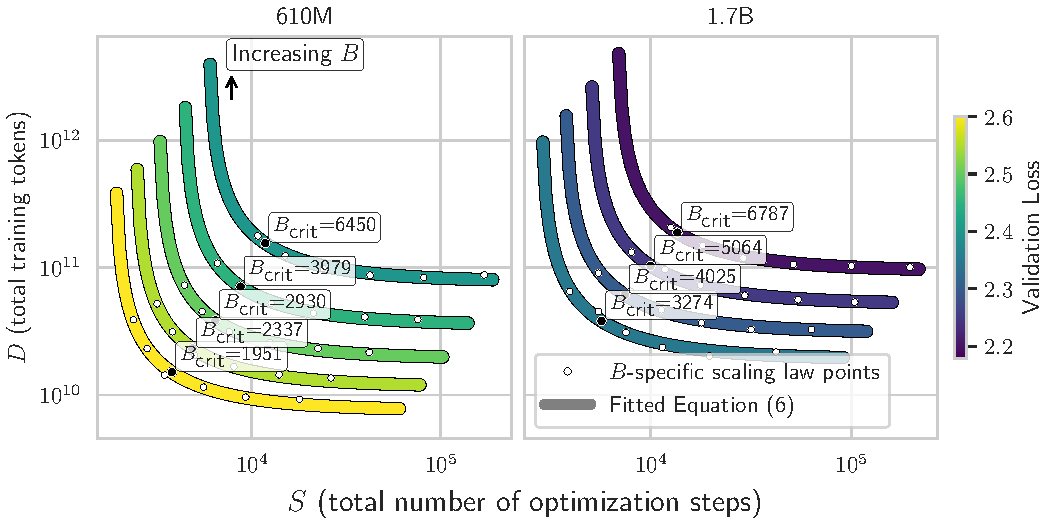
\includegraphics[trim={0.1cm 0.1cm 0.1cm 0.1cm}, clip, width=\textwidth]{pdffigs/loss_data.241005_batchsizes.twopanel_cbs.pdf}
  \caption{\textbf{\cref{eq:tradeoff} fits observed data well}:
    Increasing $B$ (moving leftward along curves) decreases
    optimization steps (x-axis), but requires more tokens (y-axis) to
    reach target loss (in color).  $\cbs$ is the transition point along
    each fitted curve.
    % Across model scales, we see that $\cbs$ does not correlate with
    % loss, but rather the number of tokens processed, $D$ (shared
    % y-axis).
    \label{fig:cbs_panels}}
%\end{figure}
